% SD-AQI paper formatted for IEEE two-column conference (IEEEtran)
\documentclass[conference]{IEEEtran}
\IEEEoverridecommandlockouts
\usepackage{graphicx}
\usepackage{amsmath}
\usepackage{amssymb}
\usepackage{siunitx}
\usepackage{cite}
\usepackage[colorlinks=true,linkcolor=blue,citecolor=blue,urlcolor=blue]{hyperref}
\usepackage{booktabs}
\sisetup{detect-all}

\title{The Scuba-Diving Air Quality Index (SD-AQI): Definition, Validation, and Application}

\author{\IEEEauthorblockN{MSc Panagiotis Nikolaou}\\
\IEEEauthorblockA{\textit{IoT Hydra Project}}}

\begin{document}
\maketitle

\begin{abstract}
We propose the Scuba-Diving Air Quality Index (SD-AQI), a compact index tailored for lightweight compressor-site monitoring. SD-AQI fuses readings from inexpensive metal-oxide semiconductor (MOS / MQ) gas sensors and environmental sensors to provide a single operational score that highlights contamination risks relevant to scuba breathing air (e.g., CO, CO$_2$, hydrocarbons, NO$_x$, NH$_3$, H$_2$). We describe the mathematical formulation, normalization, mitigation for common MOS pitfalls, and illustrative simulations and figures. The implementation captures raw payloads for forensic analysis and supports backfill and calibration.
\end{abstract}

\begin{IEEEkeywords}
Air Quality Index, MOS sensors, MQ sensors, scuba diving, SD-AQI, compressed air safety
\end{IEEEkeywords}

\section{Introduction}
Breathing-air quality in scuba diving cylinders is critical for diver safety. Contaminants such as carbon monoxide (CO), high carbon dioxide (CO$_2$), hydrocarbons (e.g., CH$_4$), volatile organic compounds (VOCs), nitrogen oxides (NO$_x$), ammonia (NH$_3$), and hydrogen (H$_2$) present significant health hazards when present at elevated concentrations. Continuous monitoring at compressor sites permits early detection and operational alarms.

Low-cost MOS (MQ) sensors are frequently used for continuous monitoring due to their sensitivity and low cost. However, MOS sensors are semiquantitative and suffer from cross-sensitivity, baseline drift, and environmental confounders. SD-AQI is designed as a pragmatic, robust operational metric that aggregates multiple sensor channels into a single scalar score optimized for early warning.

\section{Sensor Suite and Data Model}
The SD-AQI system (implemented in the IoT Babar project) collects the following channels (keys shown as stored in the database): LPG (MQ-2), CO (MQ-2,MQ-7,MQ-9), Smoke (MQ-2), CO\_MQ7 (MQ-7), CH4 (MQ-4), CO\_MQ9 (MQ-9), CO2 (MQ-135), NH3 (MQ-135), NOx (MQ-135), Alcohol/Benzene (MQ-135), H2 (MQ-8), Air (MQ-8/MQ-135), and Temperature/Humidity.

Each record $r(t)$ contains sensor values $x_g(t)$ for each gas sensor $g$ and server-side UTC timestamp $t$. The backend stores a \texttt{raw\_payload} JSON text column for every incoming record to support backfilling and forensic reprocessing.

\section{SD-AQI Formulation}
We proceed in three steps: per-gas normalization, weighting, and aggregation.

\subsection{Per-gas normalization}
For each sensor channel $g$ we compute a normalized sub-score $s_g\in[0,1]$ via a clamped linear transform:
\begin{equation}
s_g = \operatorname{clamp}\left(\frac{x_g - b_g}{u_g - b_g}, 0, 1\right)
\label{eq:normalize}
\end{equation}
where $b_g$ is a baseline (clean air) reference and $u_g$ an upper-concern threshold. The clamp function ensures $s_g$ remains in $[0,1]$. Calibration determines $b_g$ and $u_g$ (manufacturer guidance or local reference measurements).

\subsection{Weighting and aggregation}
Assign a weight $w_g \ge 0$ for each gas reflecting toxicity and operational importance. SD-AQI is then a weighted sum scaled to a convenient range:
\begin{equation}
\mathrm{SD\text{-}AQI} = C \sum_{g} w_g \; s_g
\label{eq:sd_aqi}
\end{equation}
where constant $C$ sets the numerical range (e.g., $C=6$ in the prototype). Example weights (heuristic) used in the IoT Babar implementation:
\begin{align*}
w_{CO} &= 0.05,\quad w_{CO\_MQ7} = 0.1,\quad w_{CO\_MQ9}=0.1,\\
w_{CH4} &= 0.1,\quad w_{H2}=0.05,\\
w_{CO2} &= 0.5,\quad w_{NOx}=0.1,\quad w_{Air}=0.05.
\end{align*}

When multiple sensors provide redundant information for the same gas (e.g., CO reported by MQ-2, MQ-7, MQ-9), we apply a robust fusion step: compute normalized sub-scores for each sensor and combine them via median or trimmed mean before applying a single gas-level weight. This reduces single-sensor noise influence.

\section{Handling Sensor Pitfalls}
MOS sensors exhibit several non-ideal behaviors:
\begin{itemize}
  \item \textbf{Warm-up:} sensors require heating; ignore or down-weight first N minutes after power-on.
  \item \textbf{Baseline drift:} use a rolling baseline estimator (percentile-based or exponential smoothing) to adapt $b_g$.
  \item \textbf{Humidity and temperature sensitivity:} apply compensation using measured T/H or conditional thresholds.
  \item \textbf{Cross-sensitivity:} use redundancy and statistical methods (PCA/ICA) or down-weight correlated channels.
\end{itemize}

\section{Illustrative Simulations}
We provide two illustrative plots: (1) SD-AQI response to increasing CO and (2) a simulated time-series of multiple channels and resulting SD-AQI. The prototype Python snippet (included in the project) demonstrates parameter choices and produces the figures.

Figure~\ref{fig:sd_vs_co} shows the SD-AQI as CO increases under linear normalization and the weights above. Figure~\ref{fig:sd_timeseries} shows a 30-minute synthetic trace.

\begin{figure}[!t]
\centering
\includegraphics[width=\columnwidth]{research/figures/sd_aqi_vs_co.pdf}
\caption{Illustrative SD-AQI response as CO increases (synthetic).}
\label{fig:sd_vs_co}
\end{figure}

\begin{figure}[!t]
\centering
\includegraphics[width=\columnwidth]{research/figures/sd_aqi_timeseries.pdf}
\caption{Simulated time series of gas channels and the resulting SD-AQI (synthetic).}
\label{fig:sd_timeseries}
\end{figure}

\section{Thresholds, Interpretation and Alarms}
SD-AQI is an operational indicator. Example conservative thresholds (subject to local calibration):
\begin{itemize}
  \item SD-AQI $<$ 3.0: Normal
  \item $3.0 \le$ SD-AQI $<$ 6.0: Advisory — increase inspection frequency
  \item $6.0 \le$ SD-AQI $<$ 12.0: Warning — consider stopping fills
  \item SD-AQI $\ge$ 12.0: Critical — stop filling and investigate immediately
\end{itemize}

Thresholds must be validated against reference analyzers and local safety standards. Because MOS sensors do not measure absolute concentration reliably without calibration, pair SD-AQI alarms with confirmatory measurements.

\section{Limitations and Future Work}
This work is exploratory. Limitations include the semiquantitative nature of MOS sensors and the necessity of local calibration. Future directions:
\begin{itemize}
  \item Formal calibration studies against laboratory-grade gas analyzers to map raw sensor units to concentration and set $u_g$ thresholds.
  \item Machine-learning-based compensation for cross-sensitivity and environmental confounders.
  \item Incorporating particulate measurements (PM2.5) in alarm logic and integrating with human factors for actionable alarms.
  \item Publishing reproducible notebooks and adding automated backfill utilities that extract and re-process \texttt{raw\_payload} to populate new DB columns.
\end{itemize}

\section{Conclusion}
SD-AQI provides a compact, actionable index for compressor-site monitoring. By combining multiple MOS channels with normalization, robust fusion, and weighting tuned for diving hazards, SD-AQI supports continuous monitoring and operational alarms. The approach is low-cost and enables distributed monitoring, but must be validated with reference instrumentation before use in life-critical decisions.

\section*{Acknowledgment}
The authors thank contributors to the IoT Babar project and field partners for testing and feedback.

\begin{thebibliography}{1}
\bibitem{EPAaqi} U.S. EPA, "Air Quality Index (AQI) Basics".
\bibitem{MQdatasheets} MQ series datasheets (MQ-2, MQ-4, MQ-7, MQ-8, MQ-9, MQ-135).
\end{thebibliography}

\end{document}
% SD-AQI paper formatted for IEEE two-column conference (IEEEtran)
% Note: SVG figures are referenced; convert them to PDF/PNG for pdflatex as needed.
\documentclass[conference]{IEEEtran}
\IEEEoverridecommandlockouts
\usepackage{graphicx}
\usepackage{amsmath}
\usepackage{amssymb}
\usepackage{siunitx}
\usepackage{cite}
\usepackage[colorlinks=true,linkcolor=blue,citecolor=blue,urlcolor=blue]{hyperref}
% If you want to include SVG directly, the 'svg' package + inkscape is needed; many workflows convert SVG->PDF.
% \usepackage{svg}

	itle{The Scuba-Diving Air Quality Index (SD-AQI): \newline Definition, Validation, and Application}

\author{\IEEEauthorblockN{IoT Babar Team}\\
\IEEEauthorblockA{\textit{IoT Babar Project}}}

\begin{document}
\maketitle

\begin{abstract}
We propose the Scuba-Diving Air Quality Index (SD-AQI), a compact index tailored for lightweight compressor-site monitoring. SD-AQI fuses readings from inexpensive metal-oxide semiconductor (MOS / MQ) gas sensors and environmental sensors to provide a single operational score that highlights contamination risks relevant to scuba breathing air (e.g., CO, CO$_2$, hydrocarbons, NO$_x$, NH$_3$, H$_2$). We describe the mathematical formulation, normalization, mitigation for common MOS pitfalls, and illustrative simulations and figures. The implementation captures raw payloads for forensic analysis and supports backfill and calibration.
\end{abstract}

\begin{IEEEkeywords}
Air Quality Index, MOS sensors, MQ sensors, scuba diving, SD-AQI, compressed air safety
\end{IEEEkeywords}

\section{Introduction}
Breathing-air quality in scuba diving cylinders is critical for diver safety. Contaminants such as carbon monoxide (CO), high carbon dioxide (CO$_2$), hydrocarbons (e.g., CH$_4$), volatile organic compounds (VOCs), nitrogen oxides (NO$_x$), ammonia (NH$_3$), and hydrogen (H$_2$) present significant health hazards when present at elevated concentrations. Continuous monitoring at compressor sites permits early detection and operational alarms.

Low-cost MOS (MQ) sensors are frequently used for continuous monitoring due to their sensitivity and low cost. However, MOS sensors are semiquantitative and suffer from cross-sensitivity, baseline drift, and environmental confounders. SD-AQI is designed as a pragmatic, robust operational metric that aggregates multiple sensor channels into a single scalar score optimized for early warning.

\section{Sensor Suite and Data Model}
The SD-AQI system (implemented in the IoT Babar project) collects the following channels (keys shown as stored in the database): LPG (MQ-2), CO (MQ-2,MQ-7,MQ-9), Smoke (MQ-2), CO\_MQ7 (MQ-7), CH4 (MQ-4), CO\_MQ9 (MQ-9), CO2 (MQ-135), NH3 (MQ-135), NOx (MQ-135), Alcohol/Benzene (MQ-135), H2 (MQ-8), Air (MQ-8/MQ-135), and Temperature/Humidity.

Each record $r(t)$ contains sensor values $x_g(t)$ for each gas sensor $g$ and server-side UTC timestamp $t$. The backend stores a \texttt{raw\_payload} JSON text column for every incoming record to support backfilling and forensic reprocessing.

\section{SD-AQI Formulation}
We proceed in three steps: per-gas normalization, weighting, and aggregation.

\subsection{Per-gas normalization}
For each sensor channel $g$ we compute a normalized sub-score $s_g\in[0,1]$ via a clamped linear transform:
\begin{equation}
s_g = \operatorname{clamp}\left(\frac{x_g - b_g}{u_g - b_g}, 0, 1\right)
\label{eq:normalize}
\end{equation}
where $b_g$ is a baseline (clean air) reference and $u_g$ an upper-concern threshold. The clamp function ensures $s_g$ remains in [0,1]. Calibration determines $b_g$ and $u_g$ (manufacturer guidance or local reference measurements).

\subsection{Weighting and aggregation}
Assign a weight $w_g \ge 0$ for each gas reflecting toxicity and operational importance. SD-AQI is then a weighted sum scaled to a convenient range:
\begin{equation}
\mathrm{SD\text{-}AQI} = C \sum_{g} w_g \; s_g
\label{eq:sd_aqi}
\end{equation}
where constant $C$ sets the numerical range (e.g., $C=6$ in the prototype). Example weights (heuristic) used in the IoT Babar implementation:
\begin{align*}
w_{CO} &= 0.05,\quad w_{CO\_MQ7} = 0.1,\quad w_{CO\_MQ9}=0.1,\\
w_{CH4} &= 0.1,\quad w_{H2}=0.05,\\
w_{CO2} &= 0.5,\quad w_{NOx}=0.1,\quad w_{Air}=0.05.
\end{align*}

When multiple sensors provide redundant information for the same gas (e.g., CO reported by MQ-2, MQ-7, MQ-9), we apply a robust fusion step: compute normalized sub-scores for each sensor and combine them via median or trimmed mean before applying a single gas-level weight. This reduces single-sensor noise influence.

\section{Handling Sensor Pitfalls}
MOS sensors exhibit several non-ideal behaviors:
\begin{itemize}
  \item \textbf{Warm-up:} sensors require heating; ignore or down-weight first N minutes after power-on.
  \item \textbf{Baseline drift:} use a rolling baseline estimator (percentile-based or exponential smoothing) to adapt $b_g$.
  \item \textbf{Humidity and temperature sensitivity:} apply compensation using measured T/H or conditional thresholds.
  \item \textbf{Cross-sensitivity:} use redundancy and statistical methods (PCA/ICA) or down-weight correlated channels.
\end{itemize}

\section{Illustrative Simulations}
We provide two illustrative plots: (1) SD-AQI response to increasing CO and (2) a simulated time-series of multiple channels and resulting SD-AQI. The prototype Python snippet (included in the project) demonstrates parameter choices and produces the figures.

Figure~\ref{fig:sd_vs_co} shows the SD-AQI as CO increases under linear normalization and the weights above. Figure~\ref{fig:sd_timeseries} shows a 30-minute synthetic trace.

\begin{figure}[!t]
\centering
\includegraphics[width=\columnwidth]{figures/sd_aqi_vs_co.pdf}
\caption{Illustrative SD-AQI response as CO increases (synthetic). Convert the SVG to PDF/PNG for LaTeX compilation if needed.}
\label{fig:sd_vs_co}
\end{figure}

\begin{figure}[!t]
\centering
\includegraphics[width=\columnwidth]{figures/sd_aqi_timeseries.pdf}
\caption{Simulated time series of gas channels and the resulting SD-AQI (synthetic).}
\label{fig:sd_timeseries}
\end{figure}

\section{Thresholds, Interpretation and Alarms}
SD-AQI is an operational indicator. Example conservative thresholds (subject to local calibration):
\begin{itemize}
  \item SD-AQI $<$ 3.0: Normal
  \item 3.0 $\le$ SD-AQI $<$ 6.0: Advisory — increase inspection frequency
  \item 6.0 $\le$ SD-AQI $<$ 12.0: Warning — consider stopping fills
  \item SD-AQI $\ge$ 12.0: Critical — stop filling and investigate immediately
\end{itemize}

Thresholds must be validated against reference analyzers and local safety standards. Because MOS sensors do not measure absolute concentration reliably without calibration, pair SD-AQI alarms with confirmatory measurements.

\section{Limitations and Future Work}
This work is exploratory. Limitations include the semiquantitative nature of MOS sensors and the necessity of local calibration. Future directions:
\begin{itemize}
  \item Formal calibration studies against laboratory-grade gas analyzers to map raw sensor units to concentration and set $u_g$ thresholds.
